\documentclass{article}
\usepackage[utf8]{inputenc}
\usepackage{amsmath}
\usepackage{graphicx}
\usepackage{titling}

\title{\textbf{\Huge NLP Assignment 1: Research}}
\author{Name: Alireza Dastmalchi Saei}
\date{Stu No.: 993613026}

\pretitle{%
  \begin{center}
  
\includegraphics[width = 150px]{Images/university-of-isfahan-logo.png}\\[\bigskipamount]
  \vspace{3cm}
}
\posttitle{\end{center}}

\begin{document}
\maketitle

\pagebreak

\section{Text Summarization}
Text Summarization is a natural language processing (NLP) task that involves condensing a lengthy text document into a shorter, more compact version while still retaining the most important information and meaning. The goal is to produce a summary that accurately represents the content of the original text in a concise form.\\\\
There are different approaches to text summarization:
\begin{itemize}
  \item \textbf{Extractive methods} that identify and extract important sentences or phrases from the text.
  \item \textbf{Abstractive methods} that generate new text based on the content of the original text.
\end{itemize}
\pagebreak

\section{Sentiment Analysis}
Sentiment analysis is a natural language processing (NLP) technique used to determine whether data is positive, negative or neutral. Sentiment analysis is often performed on textual data to help businesses monitor brand and product sentiment in customer feedback, and understand customer needs. Statistical machine learning models like following are used in sentiment analysis tasks:
\begin{itemize}
  \item Naive Bayes Classifier
  \item Support Vector Machine (SVM)
  \item Logistic Regression
  \item Random Forest
  \item Gradient Boosting Machines (GBM)
\end{itemize}

\pagebreak

\section{Machine Translation}
Machine translation (MT) in natural language processing (NLP) refers to the automated process of translating text or speech from one language to another. The primary goal of machine translation is to enable communication between people who speak different languages by automatically converting text or speech from a source language into an equivalent text or speech in a target language. There are 4 types of machine translation:
\begin{itemize}
  \item Statistical Machine Translation (SMT)
  \item Rule-based Machine Translation (RBMT)
  \item Hybrid Machine Translation (HMT)
  \item Neural Machine Translation (NMT)
\end{itemize}
\pagebreak

\section{Article: Abstractive Summarization Guided by Latent Hierarchical Document Structure}

\subsection{Problem Statement and Idea}
This article talks about the issue of sequential summarization methods failing to utilize the underlying structure and dependencies within the input text, leading to suboptimal summarization quality. The proposed solution aims to overcome this limitation by introducing a novel Hierarchical Graph Neural Network (HierGNN) model for abstractive summarization. The key idea is to extract the hierarchical structure of the document and inter-sentence dependencies to improve the coherence and informativeness of generated abstract summaries. This graph is learns the hierarchical structure of text via a sparse variant of the matrix-tree computation. It then formulates sentence-level
reasoning as a graph propagation problem. The proposed method is incorporated into BART and Pointer-Generator Networks (PGN) resulting an improvement on performance because HierGNN encourages the summarizers to focus on sentence fusion more than sentence compression.

\subsection{Proposed Model}
Sequential models encode an N-token-article $X = (x_1, ..., x_n)$ as a d-dimensional latent vector using an encoding function then it is decoded into target summary Y. The Hierarchy-aware Graph Neural Encoder model learns the documents structure and it consists of several key components:
\begin{enumerate}
    \item \textbf{Learning the Latent Hierarchical Structure}: HierGNN learns the hierarchical document structure without direct supervision, using a sparse variant of the matrix-tree theorem. It represents the document as a complete weighted graph, where each node represents a sentence and a root value of that sentence representing the hierarchical role of the sentence, and edge weights indicate directional dependencies between sentences.
    \item \textbf{Reasoning by Hierarchy-aware Message Passing}: HierGNN utilizes a novel message-passing mechanism over the learned hierarchical graph to propagate information between sentences, enabling inter-sentence reasoning. For the i-th sentence node, the edge marginal controls the aggregation from its
        K information nodes; and root probability controls the combined neighboring information in i-th node as $u^{(l)}$ in the l-th reasoning layer: $$u_i^{(l)} = (1 - p_i^r) . F_r(s_i^{(l)}) + (p_i^r) . \sum_{k=1}^{K} A_{ik}F_n(s_k^{(l)})$$ Where $F_r$ and $F_n$ are parametric functions. A gated mechanism is used for filtering out unnecessary information which involves calculating sigmoid and layer normalization (LN) steps.
    \item \textbf{Reasoning Fusion Layer}: This model stack L HierGNNs together where fusion layer is used for aggregating the output from each reasoning hop. There are 2 approaches for layers use:
        \begin{enumerate}
          \item Layer-Shared Reasoning (LSR): Uses a shared reasoning graph first, followed by L message passing layers for reasoning
          \item Layer-Independent Reasoning (LIR): Uses layer-wise latent hierarchical graphs independently, where each message passing layer uses its own graph
        \end{enumerate}
    \item \textbf{Graph-selection Attention Mechanism}: HierGNN incorporates a graph-selection attention mechanism to inform the decoder with learned hierarchical information during decoding, improving the relevance and coherence of generated summaries.
\end{enumerate}

\begin{figure}[h]
  \centering
  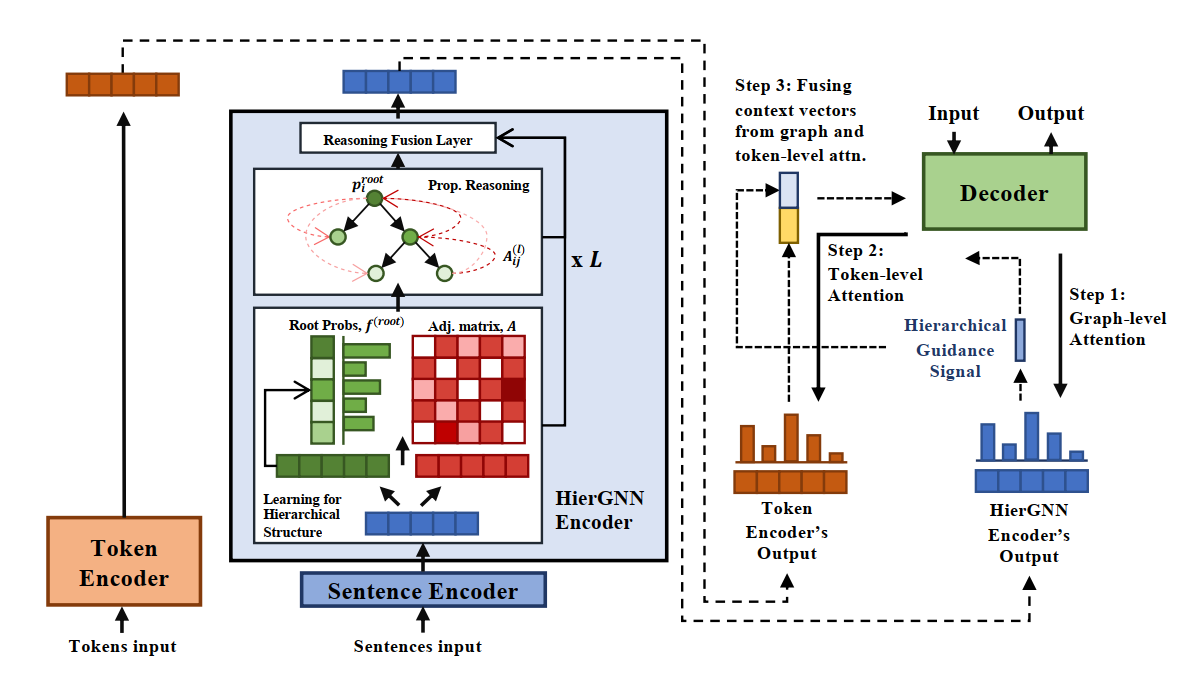
\includegraphics[width=1\textwidth]{Images/Model.png}
  \caption{Architecture for the sequence-to-sequence model with HierGNN reasoning encoder.}
  \label{fig:model_diagram}
\end{figure}

\pagebreak

\subsection{Results}
The experimental results demonstrate the effectiveness of the proposed HierGNN model:
\begin{itemize}
    \item \textbf{Automatic Evaluation}: HierGNN achieves significant improvements in ROUGE F-1 scores compared to baseline models, both for non-pretrained and pretrained summarizers on datasets CNN/DM, XSum, and PubMed. Additionally, the HierGNN-PGN model outperforms StructSum ES and ES+IS, which explicitly construct document-level graph representations using external parsers.
    \item \textbf{Human Evaluations}: Human referees (from Amazon Mechanical Turk) assess HierGNN-BART as producing the overall best summaries in terms of \textbf{relevance}, \textbf{informativeness}, and \textbf{redundancy}, compared to other abstractive baselines such as BERTSUMABS, T5-Large, and BART.
    \item \textbf{Ablations}: Ablation studies confirm the positive contribution of HierGNN components, including the reasoning module, graph-selection attention, sparse matrix-tree computation, and graph fusion layer, to the overall performance of the model in summarization tasks.
\end{itemize}


\end{document}
